\documentclass[12pt,a4paper]{article}

% ─── Page Layout ───────────────────────────────────────────────────────────────
\usepackage[a4paper, margin=0.8in, headheight=14pt]{geometry}

% ─── Fonts (XeLaTeX) ───────────────────────────────────────────────────────────
\usepackage{fontspec}
\usepackage{unicode-math}
\setmainfont{TeX Gyre Pagella}
\setmonofont[Scale=0.88]{TeX Gyre Cursor}
\setmathfont{Latin Modern Math}

% ─── Packages ──────────────────────────────────────────────────────────────────
\usepackage{xcolor}
\usepackage{colortbl}
\usepackage{titlesec}
\usepackage{enumitem}
\usepackage{tabularx}
\usepackage{booktabs}
\usepackage{array}
\usepackage{amsmath}
\usepackage{tikz}
\usetikzlibrary{shapes.geometric, arrows.meta, positioning, calc, fit, decorations.pathreplacing}
\usepackage{tcolorbox}
\tcbuselibrary{skins, breakable}
\usepackage{hyperref}
\usepackage{fancyhdr}
\usepackage{graphicx}
\usepackage{microtype}
\hyphenpenalty=10000
\exhyphenpenalty=10000
\sloppy
\usepackage{caption}
\usepackage{setspace}
\usepackage{multirow}
\usepackage{tocloft}

% ─── Q&A helper ────────────────────────────────────────────────────────────────
\newcommand{\Q}[1]{\textbf{#1}\par\noindent\ignorespaces}

% ─── Colour Palette ────────────────────────────────────────────────────────────
\definecolor{myred}{RGB}{196,30,58}
\definecolor{mydark}{RGB}{30,30,50}
\definecolor{mygreen}{RGB}{14,120,80}
\definecolor{myteal}{RGB}{0,130,140}
\definecolor{myamber}{RGB}{180,100,0}
\definecolor{mypurple}{RGB}{100,30,160}
\definecolor{mygray}{RGB}{246,247,249}
\definecolor{mgframe}{RGB}{180,185,200}
\definecolor{watermark}{RGB}{145,150,170}
\definecolor{hdrred}{RGB}{250,232,235}
\definecolor{hdrgreen}{RGB}{220,244,233}
\definecolor{hdrteal}{RGB}{220,242,244}
\definecolor{hdramber}{RGB}{253,242,215}
\definecolor{hdrpurple}{RGB}{238,228,255}
\definecolor{hdrgray}{RGB}{238,240,245}
\definecolor{rowalt}{RGB}{250,251,253}

% ─── Section Formatting ────────────────────────────────────────────────────────
\titleformat{\section}
  {\large\bfseries\color{myred}}{\thesection.}{0.5em}{}
  [\vspace{1pt}{\color{myred}\rule{\linewidth}{0.8pt}}]
\titleformat{\subsection}
  {\normalsize\bfseries\color{myteal}}{\thesubsection}{0.5em}{}
\titlespacing*{\section}{0pt}{18pt}{7pt}
\titlespacing*{\subsection}{0pt}{11pt}{4pt}

% ─── Paragraph ─────────────────────────────────────────────────────────────────
\setlength{\parindent}{0pt}
\setlength{\parskip}{4pt}

% ─── TOC Styling ───────────────────────────────────────────────────────────────
\renewcommand{\cfttoctitlefont}{\large\bfseries\color{myred}}
\renewcommand{\cftaftertoctitle}{\par\noindent{\color{myred}\rule{\linewidth}{0.8pt}}}
\setlength{\cftbeforetoctitleskip}{0pt}
\setlength{\cftaftertoctitleskip}{6pt}
\renewcommand{\cftsecfont}{\normalsize\bfseries\color{mydark}}
\renewcommand{\cftsecpagefont}{\normalsize\bfseries\color{mydark}}
\renewcommand{\cftsecleader}{\cftdotfill{\cftdotsep}}
\setlength{\cftbeforesecskip}{7pt}
\renewcommand{\cftsubsecfont}{\small\color{mydark}}
\renewcommand{\cftsubsecpagefont}{\small\color{mydark}}
\setlength{\cftbeforesubsecskip}{3pt}
\setlength{\cftsubsecindent}{1.4em}

% ─── Table helpers ─────────────────────────────────────────────────────────────
\renewcommand{\arraystretch}{1.45}
\setlength{\tabcolsep}{6pt}
\arrayrulecolor{mydark}
\newcolumntype{B}[1]{>{\small\bfseries\raggedright\arraybackslash}m{#1}}
\newcolumntype{Y}{>{\small\raggedright\arraybackslash}X}
\renewcommand{\tabularxcolumn}[1]{m{#1}}

% ─── Header / Footer ───────────────────────────────────────────────────────────
\pagestyle{fancy}
\fancyhf{}
\fancyhead[L]{\small\color{myred}\textbf{PE-EC702B}\;\color{mydark}--- Digital Image and Video Processing}
\fancyhead[R]{\small\color{myteal}\textbf{Module 3 Notes}}
\fancyfoot[C]{\small\color{mydark}\thepage}
\fancyfoot[R]{\small\color{watermark}\textit{\copyright\ Biraj}}
\renewcommand{\headrulewidth}{0.5pt}
\renewcommand{\footrulewidth}{0.3pt}

% ─── Hyperref ──────────────────────────────────────────────────────────────────
\hypersetup{
  colorlinks=true, linkcolor=myteal, urlcolor=myteal,
  pdfauthor={Biraj Sarkar},
  pdftitle={PE-EC702B --- Module 3 Notes}
}

% ─── tcolorbox styles ──────────────────────────────────────────────────────────
\tcbset{
  tikzbox/.style={
    colback=mygray, colframe=mgframe, boxrule=0.6pt, arc=4pt,
    left=8pt, right=8pt, top=6pt, bottom=6pt,
    colbacktitle=mgframe, coltitle=mydark,
    fonttitle=\small\bfseries
  },
  defbox/.style={
    colback=hdrgreen, colframe=mygreen, boxrule=0.8pt, arc=4pt,
    left=9pt, right=9pt, top=6pt, bottom=6pt,
    colbacktitle=mygreen, coltitle=white,
    fonttitle=\small\bfseries
  },
  formulabox/.style={
    colback=hdrteal, colframe=myteal, boxrule=0.8pt, arc=4pt,
    left=9pt, right=9pt, top=7pt, bottom=7pt,
    colbacktitle=myteal, coltitle=white,
    fonttitle=\small\bfseries
  },
  examplebox/.style={
    colback=hdramber, colframe=myamber, boxrule=0.8pt, arc=4pt,
    left=9pt, right=9pt, top=6pt, bottom=6pt,
    colbacktitle=myamber, coltitle=white,
    fonttitle=\small\bfseries,
    breakable
  },
  masonbox/.style={
    colback=hdrpurple, colframe=mypurple, boxrule=0.8pt, arc=4pt,
    left=9pt, right=9pt, top=6pt, bottom=6pt,
    colbacktitle=mypurple, coltitle=white,
    fonttitle=\small\bfseries
  },
  exambox/.style={
    colback=hdrpurple, colframe=mypurple, boxrule=1pt, arc=5pt,
    left=10pt, right=10pt, top=8pt, bottom=8pt,
    colbacktitle=mypurple, coltitle=white,
    fonttitle=\bfseries,
    breakable, title after break={\textbf{Frequently Asked / Viva Questions (contd.)}}}
}
\tcbset{breakable}

% ─── TikZ styles ───────────────────────────────────────────────────────────────
\tikzset{
  block/.style={rectangle, draw=myteal, fill=hdrteal,
    text width=2.1cm, align=center, minimum height=0.85cm,
    font=\small, rounded corners=3pt, line width=0.7pt},
  arrow/.style={-Stealth, thick, color=mydark},
  line/.style={thick, color=mydark}
}

% ═══════════════════════════════════════════════════════════════════════════════
\begin{document}
% ═══════════════════════════════════════════════════════════════════════════════

\begin{center}
  {\LARGE\bfseries\color{myred} PE-EC702B --- Digital Image and Video Processing}\\[5pt]
  {\normalsize\color{mydark} Semester VII \quad$\bullet$\quad 3L:0T:0P \quad$\bullet$\quad 3 Credits}\\[3pt]
  {\normalsize\color{myteal}\textbf{Module 3 Exam Notes: Color Image Processing}}\\[3pt]
  {\small\color{mydark} CGEC \;$|$\; B.Tech ECE (2023--27) \;$|$\; \textit{Biraj Sarkar}}
\end{center}
\vspace{2pt}
\noindent{\color{myred}\rule{\linewidth}{1.5pt}}
\vspace{2pt}

\hypersetup{linkcolor=mydark}
\tableofcontents
\hypersetup{linkcolor=myteal}
\newpage

% ===============================================================================
\section{Color Models}
% ===============================================================================

Color models provide a standardized way to specify colors. They are typically categorized as hardware-oriented (RGB, YUV) or human-oriented (HSI).

\subsection{RGB Color Model}
The RGB model is based on a 3D Cartesian coordinate system where the primary colors Red, Green, and Blue are at three corners. The values are typically normalized to $[0,1]$:
\begin{itemize}[leftmargin=*, itemsep=2pt]
  \item Black is at the origin $(0,0,0)$, while White is at $(1,1,1)$.
  \item Colors are additive: combining primaries yields secondary colors (Cyan, Magenta, Yellow).
\end{itemize}

\subsection{YUV Color Model}
Used widely in television transmission and video compression standards (like MPEG/H.26X). It decouples brightness (Luminance) from color (Chrominance):
\begin{itemize}[leftmargin=*, itemsep=3.5pt]
  \item \textbf{Y (Luminance):} Represents brightness information.
  \item \textbf{U and V (Chrominance):} Represent color differences.
  \item Conversion from RGB to YUV:
    \begin{align}
      Y &= 0.299R + 0.587G + 0.114B \\
      U &= -0.14713R - 0.28886G + 0.436B \approx 0.492(B - Y) \\
      V &= 0.615R - 0.51499G - 0.10001B \approx 0.877(R - Y)
    \end{align}
\end{itemize}

\subsection{HSI Color Model}
The HSI model decouples intensity from color-carrying information, matching human visual perception.

\begin{tcolorbox}[defbox, title={HSI Components}]
\begin{itemize}[leftmargin=*, itemsep=3pt]
  \item \textbf{Hue (H):} Describes the pure color (e.g., yellow, red, purple) represented as an angle from $0^\circ$ to $360^\circ$.
  \item \textbf{Saturation (S):} Represents the purity or dilution of the color with white (range $[0,1]$).
  \item \textbf{Intensity (I):} Represents the brightness or gray-level value (range $[0,1]$).
\end{itemize}
\end{tcolorbox}

\begin{tcolorbox}[formulabox, title={RGB to HSI Conversion Formulas}]
Given $R, G, B \in [0, 1]$, the HSI components are computed as:
\begin{align}
  I &= \frac{1}{3}(R + G + B) \\
  S &= 1 - \frac{3}{R + G + B} \left[ \min(R, G, B) \right] \\
  H &= \begin{cases} \theta & \text{if } B \le G \\ 360^\circ - \theta & \text{if } B > G \end{cases}
\end{align}
where the angle $\theta$ is:
\begin{equation}
  \theta = \cos^{-1} \left( \frac{\frac{1}{2}\left[(R - G) + (R - B)\right]}{\sqrt{(R - G)^2 + (R - B)(G - B)}} \right)
\end{equation}
\end{tcolorbox}

\begin{tcolorbox}[tikzbox, title={HSI Color Model Coordinates}]
\centering
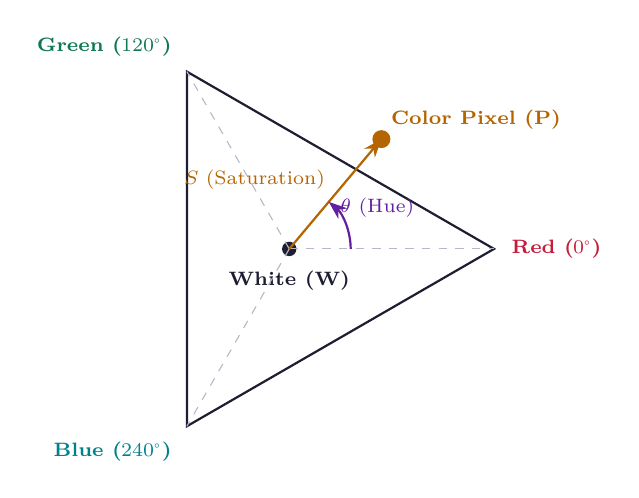
\begin{tikzpicture}[scale=1.3, every node/.style={font=\scriptsize}]
  % Draw RGB triangle on the chromaticity plane
  \draw[thick, color=mydark] (0:2) coordinate (R) -- (120:2) coordinate (G) -- (240:2) coordinate (B) -- cycle;
  
  % Label vertices
  \node[right=0.1cm, color=myred] at (R) {\textbf{Red ($0^\circ$)}};
  \node[above left=0.1cm, color=mygreen] at (G) {\textbf{Green ($120^\circ$)}};
  \node[below left=0.1cm, color=myteal] at (B) {\textbf{Blue ($240^\circ$)}};
  
  % Center point (White)
  \fill[color=mydark] (0,0) circle (2pt) node[below=0.15cm] {\textbf{White (W)}};
  
  % Draw lines from center to vertices
  \draw[dashed, color=mgframe] (0,0) -- (R);
  \draw[dashed, color=mgframe] (0,0) -- (G);
  \draw[dashed, color=mgframe] (0,0) -- (B);
  
  % Draw an arbitrary color point P
  \coordinate (P) at (50:1.4);
  \fill[color=myamber] (P) circle (2.5pt) node[above right] {\textbf{Color Pixel (P)}};
  \draw[thick, -Stealth, color=myamber] (0,0) -- (P) node[midway, above left, yshift=-2pt] {$S$ (Saturation)};
  
  % Draw Hue angle arc from 0 to 50 degrees
  \draw[thick, color=mypurple, -Stealth] (0:0.6) arc (0:50:0.6);
  \node[color=mypurple] at (25:0.95) {$\theta$ (Hue)};
\end{tikzpicture}
\end{tcolorbox}

% ===============================================================================
\section{Color Transformations}
% ===============================================================================

Color transformations map input color pixels $\mathbf{r}$ to output pixels $\mathbf{s}$:
\begin{equation}
  s_i = T_i(r_1, r_2, \dots, r_n) \quad \text{for } i = 1, 2, \dots, n
\end{equation}
where $n$ is the number of color space dimensions (e.g., $n=3$ for RGB/HSI).

\subsection{Formulations and Corrections}
\begin{itemize}[leftmargin=*, itemsep=3.5pt]
  \item \textbf{Color Complements:} Analogous to gray-scale negatives. In RGB space, the complement is obtained by subtracting the color values from the maximum:
    \begin{equation}
      s_R = 1 - r_R, \quad s_G = 1 - r_G, \quad s_B = 1 - r_B
    \end{equation}
    Useful for enhancing dark details in color images.
  \item \textbf{Color Slicing:} Highlights a specific range of colors in an image while background is set to gray. A prototype color vector $\mathbf{a}$ and distance threshold $D_0$ are defined:
    \begin{equation}
      s_i = \begin{cases} r_i & \text{if } \|\mathbf{z} - \mathbf{a}\| \le D_0 \\ 0.5 & \text{if } \|\mathbf{z} - \mathbf{a}\| > D_0 \end{cases}
    \end{equation}
  \item \textbf{Tone and Color Corrections:} Adjusting brightness, contrast, and gamma on color channels. Applying gamma correction on Intensity ($I$) in HSI space preserves the original hue and saturation, avoiding unwanted color shifts that occur when applying it directly on individual RGB channels.
\end{itemize}

% ===============================================================================
\section{Color Image Smoothing and Sharpening}
% ===============================================================================

\subsection{Color Image Smoothing}
Smoothing can be performed either in full-color vector space or by processing individual channels separately.
\par\noindent
For a neighborhood $S_{xy}$, the average vector is:
\begin{equation}
  \bar{\mathbf{c}}(x,y) = \frac{1}{K}\sum_{(s,t)\in S_{xy}} \mathbf{c}(s,t) = \begin{bmatrix}
    \frac{1}{K}\sum r_R(s,t) \\
    \frac{1}{K}\sum r_G(s,t) \\
    \frac{1}{K}\sum r_B(s,t)
  \end{bmatrix}
\end{equation}
Since vector addition is performed component-wise, smoothing each RGB channel independently yields the exact same result as full-color vector smoothing.

\subsection{Color Image Sharpening}
Sharpening utilizes the Laplacian operator. In RGB vector space:
\begin{equation}
  \nabla^2 \mathbf{c}(x,y) = \begin{bmatrix}
    \nabla^2 c_R(x,y) \\
    \nabla^2 c_G(x,y) \\
    \nabla^2 c_B(x,y)
  \end{bmatrix}
\end{equation}
Like smoothing, color sharpening can be executed by applying the Laplacian operator independently to the Red, Green, and Blue channels.

% ===============================================================================
\section{Color Segmentation}
% ===============================================================================

Color segmentation partitions an image into regions based on color features.

\subsection{Segmentation in RGB Space}
Given a sample set of prototype pixels representing the target color, we compute their mean vector $\mathbf{a}$ and covariance matrix $\mathbf{C}$.
\begin{itemize}[leftmargin=*, itemsep=3.5pt]
  \item \textbf{Euclidean Distance Classifier:} If color features are uncorrelated, we classify pixel $\mathbf{z}$ based on Euclidean distance:
    \begin{equation}
      D(\mathbf{z}, \mathbf{a}) = \|\mathbf{z} - \mathbf{a}\| = \sqrt{(z_R - a_R)^2 + (z_G - a_G)^2 + (z_B - a_B)^2}
    \end{equation}
    A pixel is segmented if $D(\mathbf{z}, \mathbf{a}) \le D_0$.
  \item \textbf{Mahalanobis Distance Classifier:} Accounts for correlations between channels:
    \begin{equation}
      D_M(\mathbf{z}, \mathbf{a}) = \sqrt{(\mathbf{z} - \mathbf{a})^T \mathbf{C}^{-1} (\mathbf{z} - \mathbf{a})}
    \end{equation}
\end{itemize}

\subsection{Segmentation in HSI Space}
Typically performed by thresholding Hue ($H$) and Saturation ($S$) channels:
\begin{itemize}[leftmargin=*, itemsep=2pt]
  \item Intensity is often ignored, making the segmentation robust to illumination variations and shadows.
\end{itemize}

% ===============================================================================
\section{Worked Examples}
% ===============================================================================

\begin{tcolorbox}[examplebox, title={RGB to HSI Conversion}]
\textbf{Problem:} Convert the normalized RGB pixel color vector $\mathbf{c} = [0.2, 0.8, 0.4]^T$ to HSI coordinates.

\par\noindent\rule{\linewidth}{0.5pt}\par
\textbf{Solution:}
Given $R = 0.2$, $G = 0.8$, $B = 0.4$.

\textbf{1. Calculate Intensity (I):}
\begin{equation*}
  I = \frac{1}{3}(R + G + B) = \frac{1}{3}(0.2 + 0.8 + 0.4) = \frac{1.4}{3} \approx 0.467
\end{equation*}

\textbf{2. Calculate Saturation (S):}
First, find $\min(R,G,B) = \min(0.2, 0.8, 0.4) = 0.2$.
\begin{equation*}
  S = 1 - \frac{3}{R + G + B} \left[ \min(R, G, B) \right] = 1 - \frac{3}{1.4}(0.2) = 1 - \frac{0.6}{1.4} = 1 - 0.429 = 0.571
\end{equation*}

\textbf{3. Calculate Hue (H):}
First, calculate the angle $\theta$:
\begin{align*}
  \text{Numerator} &= \frac{1}{2} \left[ (R - G) + (R - B) \right] = \frac{1}{2} \left[ (0.2 - 0.8) + (0.2 - 0.4) \right] \\
  &= \frac{1}{2} \left[ -0.6 - 0.2 \right] = -0.4 \\[4pt]
  \text{Denominator} &= \sqrt{(R-G)^2 + (R-B)(G-B)} = \sqrt{(0.2-0.8)^2 + (0.2-0.4)(0.8-0.4)} \\
  &= \sqrt{(-0.6)^2 + (-0.2)(0.4)} = \sqrt{0.36 - 0.08} = \sqrt{0.28} \approx 0.529
\end{align*}
Compute $\cos\theta$:
\begin{equation*}
  \cos\theta = \frac{-0.4}{0.529} \approx -0.756
\end{equation*}
Therefore:
\begin{equation*}
  \theta = \cos^{-1}(-0.756) \approx 139.1^\circ
\end{equation*}
Since $B = 0.4$ and $G = 0.8$, we have $B \le G$. Thus, Hue is:
\begin{equation*}
  H = \theta = 139.1^\circ
\end{equation*}

\par\noindent\textbf{Final Result:}
The HSI coordinate is:
\begin{equation*}
  H = 139.1^\circ, \quad S = 0.571, \quad I = 0.467
\end{equation*}
\end{tcolorbox}

\newpage

% ===============================================================================
% MANDATORY QUICK REVISION PAGE
% ===============================================================================
\begin{center}
  {\large\bfseries\color{myred} Quick Revision --- Module III}\\[3pt]
  {\small\color{mydark} Color Image Processing $|$ PE-EC702B}
\end{center}
\noindent{\color{myred}\rule{\linewidth}{1.2pt}}
\vspace{4pt}

\begin{tcolorbox}[formulabox, title={\textbf{Key Formulas at a Glance}}]
\renewcommand{\arraystretch}{1.3}
\begin{tabularx}{\linewidth}{B{5.0cm} X}
Intensity (HSI) & $I = \frac{1}{3}(R + G + B)$ \\
Saturation (HSI) & $S = 1 - \frac{3}{R + G + B} \left[ \min(R, G, B) \right]$ \\
Luminance (YUV) & $Y = 0.299R + 0.587G + 0.114B$ \\
RGB Color Complement & $s_R = 1 - r_R, \quad s_G = 1 - r_G, \quad s_B = 1 - r_B$ \\
RGB Euclidean distance & $D(\mathbf{z}, \mathbf{a}) = \sqrt{(z_R - a_R)^2 + (z_G - a_G)^2 + (z_B - a_B)^2}$ \\
Mahalanobis distance & $D_M(\mathbf{z}, \mathbf{a}) = \sqrt{(\mathbf{z} - \mathbf{a})^T \mathbf{C}^{-1} (\mathbf{z} - \mathbf{a})}$
\end{tabularx}
\tcbset{colbacktitle=myteal, coltitle=white}
\end{tcolorbox}

\begin{tcolorbox}[defbox, title={\textbf{One-Line Definitions}}]
\begin{itemize}[leftmargin=*, itemsep=2.5pt, topsep=0pt]
  \item \textbf{Additive Color Model:} Model (like RGB) where primary light sources are added together to create other colors.
  \item \textbf{Hue:} An attribute associated with the dominant wavelength in a mixture of light waves, representing pure color.
  \item \textbf{Saturation:} A measure of the relative purity of a color, indicating how much white light is mixed with it.
  \item \textbf{Color Slicing:} A transformation that isolates a sample color band in an image by zeroing out distant color vectors.
  \item \textbf{Full-Color Processing:} Processing pixels directly as multi-dimensional color vectors rather than scalar components.
  \item \textbf{Chrominance:} The color-carrying portion of a video signal, represented by U and V components in YUV.
\end{itemize}
\end{tcolorbox}

\begin{tcolorbox}[exambox, title={\textbf{Frequently Asked / Viva Questions}}]
\begin{enumerate}[leftmargin=*, itemsep=3.5pt, label=\arabic*.]
  \item \Q{Why is the HSI color model preferred over RGB for human interface design?} Because HSI decouples intensity (brightness) from color features (hue/saturation), which mimics how the human brain perceives and describes colors.
  \item \Q{Which color model is used in video/television broadcasting? Why?} YUV (or $\text{YC}_b\text{C}_r$), because it separates luminance ($Y$) from chrominance. This allows compatible broadcasting to black-and-white TVs and compression of color bandwidth without affecting perceived quality.
  \item \Q{Can we smooth a color image by filtering RGB channels independently?} Yes. Since the average of vectors is equal to the vector containing the averages of their components, independent channel filtering produces mathematically identical results to full-color vector smoothing.
  \item \Q{What is the complement of Red in RGB space?} Under normalized RGB space, Red is $(1,0,0)$. Its complement is $(1-1, 1-0, 1-0) = (0,1,1)$, which represents Cyan (a secondary color).
  \item \Q{What is the main advantage of segmenting color images in HSI space?} By thresholding only Hue ($H$) and Saturation ($S$) and ignoring Intensity ($I$), the segmentation becomes robust to shadows and spatial variations in lighting.
  \item \Q{Explain the physical meaning of a Saturation value of 0.} A saturation of 0 means the color is completely diluted with white light, representing a neutral shade of gray.
  \item \Q{Why do we apply gamma correction to the Intensity channel in HSI rather than RGB channels?} Applying it to RGB channels independently alters their relative ratios, causing severe shifts in hue. Correcting the Intensity channel in HSI preserves hue and saturation.
  \item \Q{What is the difference between Euclidean and Mahalanobis distance in RGB segmentation?} Euclidean distance assumes all color channels are independent and have equal variance. Mahalanobis distance uses the covariance matrix to account for channel correlations.
  \item \Q{What are subtractive primary colors?} Cyan, Magenta, and Yellow. They are used in color printing and act as filters that absorb specific wavelengths of light.
  \item \Q{What does the angle $\theta$ represent in HSI?} The angle $\theta$ represents the starting hue reference vector. It is measured counterclockwise starting from the Red axis ($0^\circ$).
\end{enumerate}
\tcbset{colbacktitle=myteal, coltitle=white}
\end{tcolorbox}

\begin{tcolorbox}[tikzbox, title={Comparison of Color Models}]
\centering
\renewcommand{\arraystretch}{1.2}
\begin{tabularx}{\linewidth}{>{\bfseries}B{3.2cm} Y Y Y}
Attribute & RGB & YUV & HSI \\
\midrule
Primary Focus & Hardware (displays) & Video coding/TV & Human perception \\
Components & Red, Green, Blue & Luminance, Chrominance & Hue, Saturation, Intensity \\
Decoupled Brightness & No & Yes (via $Y$) & Yes (via $I$) \\
\bottomrule
\end{tabularx}
\tcbset{colbacktitle=myteal, coltitle=white}
\end{tcolorbox}

\end{document}
